%\documentclass[reprint,longbibliography,superscriptaddress, onecolumn, english, notitlepage]{revtex4-1}
%\documentclass[aps,prl,reprint,longbibliography]{revtex4-1}
\documentclass{article}
%\usepackage{graphicx}
 \usepackage[utf8]{inputenc}
 \usepackage{amsmath,bm}
 \usepackage{mathrsfs}
 \usepackage{amsfonts}
 %\usepackage[font=it]{caption}
 \usepackage{graphicx}
 %\usepackage{xcolor}
 \usepackage{setspace} %leaves captions single space in draft mode
 \usepackage{graphicx}
 \usepackage{epstopdf}
 \usepackage{dcolumn}
 \usepackage{amsmath}
 \usepackage{epsfig}
 \usepackage{indentfirst}
 \usepackage{psfrag}
 \usepackage[normalem]{ulem}
 \usepackage{subfigure}
 %\usepackage{subcaption}
 \usepackage{amssymb}
 %\bibliographystyle{apsrev}
\usepackage{caption}
\usepackage{color}
 \usepackage{units} % rz
\usepackage{soul} % strikethrough text
\usepackage{siunitx}
 \usepackage{graphicx}% Include figure files
 \usepackage{float}
 \graphicspath{{Figures/}} %Setting the graphicspath
 \usepackage{dcolumn}% Align table columns on decimal point
 \usepackage{bm}% bold math
 \usepackage{multirow}

\usepackage{physics}
\usepackage{dcolumn}% Align table columns on decimal point
\usepackage{bm}% bold mathhttps://www.overleaf.com/project/5af95d0f3775594d14d4a052
%\usepackage{hyperref}% add hypertext capabilities
\usepackage{natbib}
\usepackage[backref=none,bookmarksnumbered=true,bookmarks=true,bookmarksopen=true,colorlinks=true,
citecolor=blue,linkcolor=blue,anchorcolor=green,urlcolor=blue,unicode=false]{hyperref}

%******************************* For corrections ===================
\usepackage{ulem}[normalem] %Whatch out, places underlining in Journal references. Use \normalem before references to deactivate this
\def\red{\color{red}}
\def\black{\color{black}}
\def\blue{\color{blue}}
\def\BappCl{BaCl$_2$}
\def\Bapp{Ba$^{2+} \,$}


\title{Experiment proposal: high vacuum microscopy with FBI thin layers}
\author{Pablo Herrero-G\'omez, Alex Fontana}

\date{\today}
\begin{document}

\maketitle

\section{Motivation}

The NEXT collaboration is developing dry-phase Fluorescent Bicolor Indicators (FBI) for \Bapp, which is the ion daughter in the radioactive double beta decay of $^{136}$Xe. The final application of a \Bapp sensor requires identification of a molecule chelated with the ion in a High Pressure Xenon Time Projection Chamber (HPXe-TPC). Therefore, the sensor must consist of a monolayer (ML) of molecular indicators which preserve its properties of fluorescence and  affinity for barium in this regime, i.e. on the very surface of a substrate and in high pressure chamber. So far, we have proved that the molecules preserve its fluorescence in dry phase \cite{rivilla_fluorescent_2020} and that \Bapp is captured by a monolayer of FBI in UHV (paper in preparation). We have also checked the chemical stability of FBI after being exposed to air for several days. Thus, a natural next step towards the final sensor would be to prove that the fluorescence is preserved in vacuum.

In addition, we have included two further conditions in the design of the sensor substrate: it must be transparent, in order to allow measurements of microscopy in transmission, and it must be slightly conducting, in order to attract the ion towards its surface. For these reasons, we have selected a substrate of optical quartz coated with several ITO layers. However, any conducting surface induces quenching of a fluorescent signal. Some models indicate that, in this scenario, the fluorescence photons are emitted towards the inner layers of the substrate. An experiment to confirm or deny this hypothesis is therefore crucial for our purposes.

Lastly, let us note that that the final goal is to be able to detect Single Molecule Fluorescence (SMF) of a chelated molecule emitting in blue surrounded by a large number of unchelated molecules emitting in green (orange/red for new generations of the molecule that the collaboration is investigating in parallel). For this reason, the investigation of different detection technologies is desirable. In particular, single-photon counting APDs could represent an attractive possibility to increase the sensitivity.

\section{Setup description}

\begin{figure*}[ht!]
	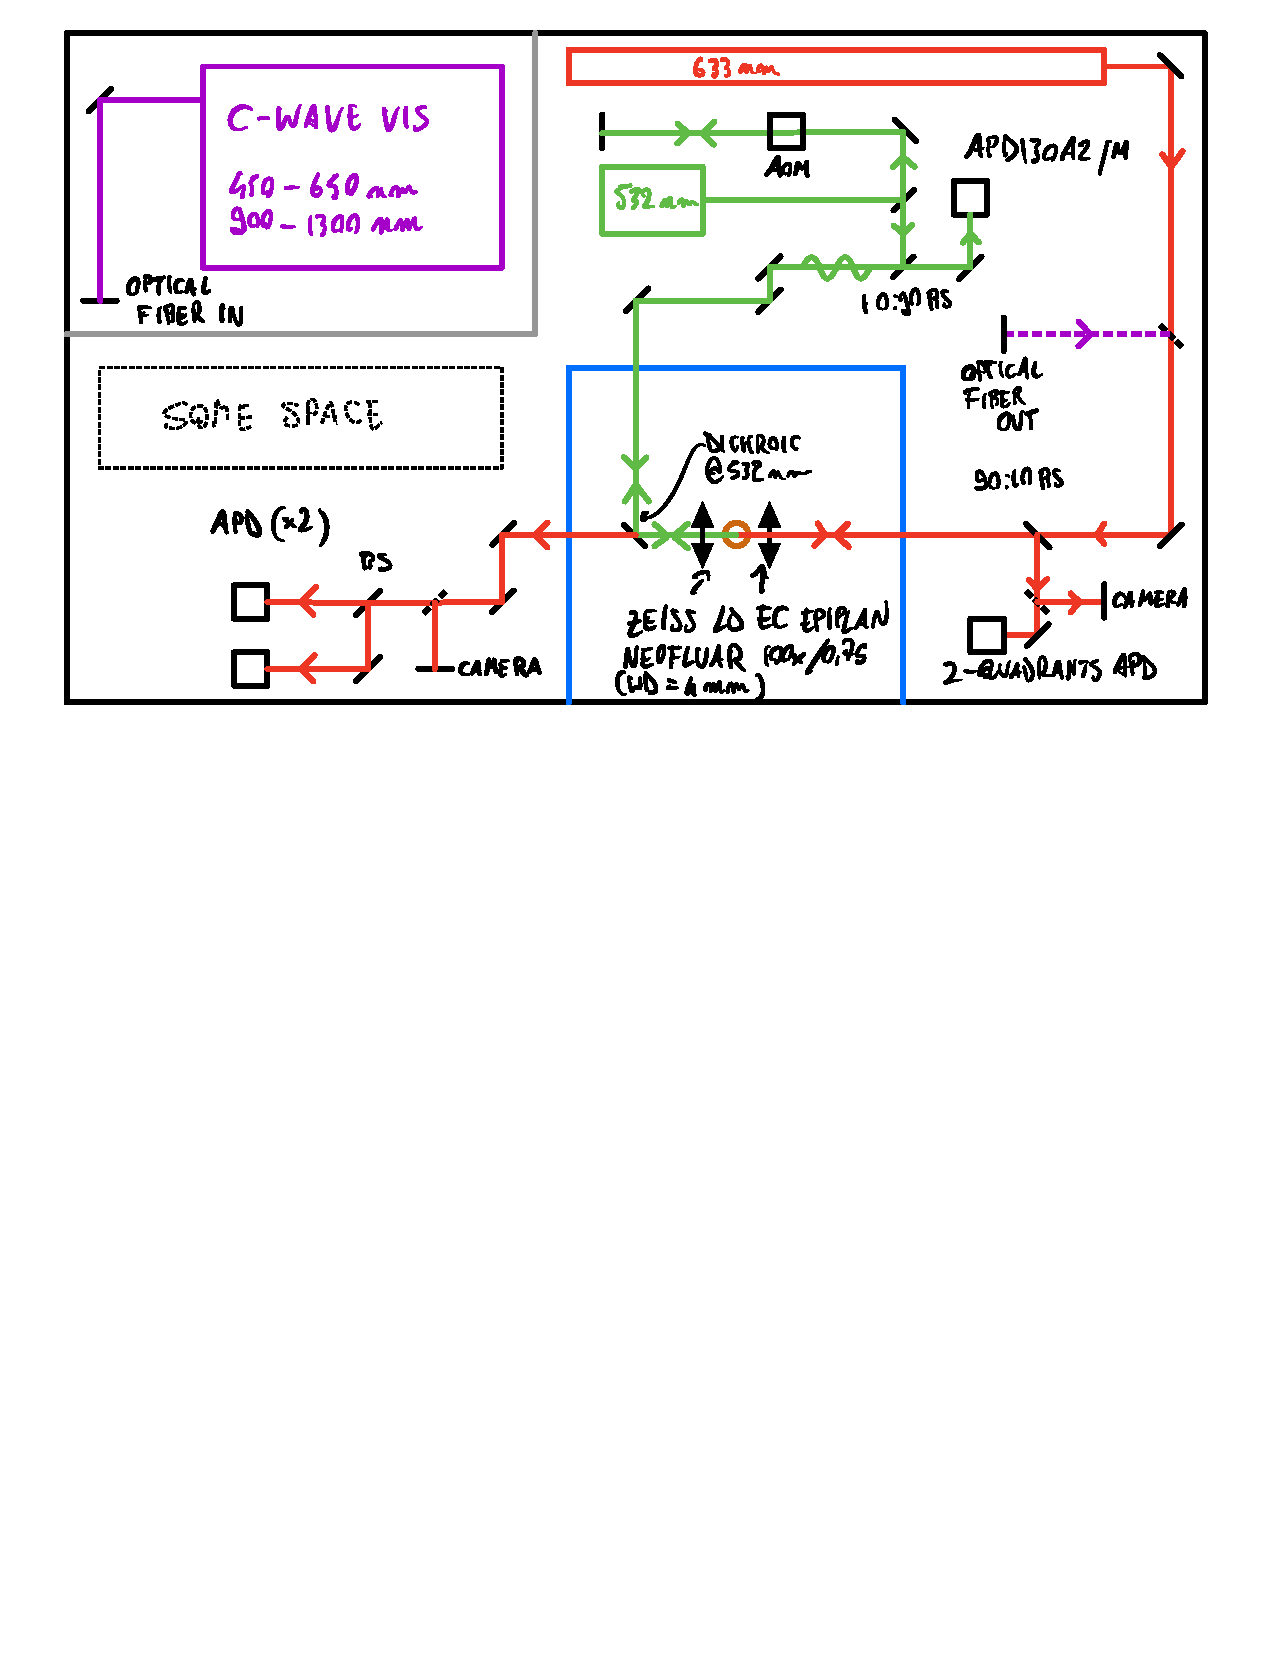
\includegraphics[width=0.95\textwidth]{figures/Schema.pdf}
	\caption{\label{figSetup1} Optical setup under construction in the Institut N\'eel.}
\end{figure*}

Figure \ref{figSetup1} shows a sketch of the setup under construction in the Institut N\'eel by A. Fontana under the supervision of B. Pigeau and O. Arcizet. The goal of the experiment is to measure the  interaction of a silicon carbide nanowire and a NV center, which acts as a quantum two-level system. The mechanical movement of the nanowire is read thanks to a $\lambda=\SI{633}{\nano m}$ laser reading in reflection by a two-quadrant photodiode (QPD). The NV center is pumped by a $\lambda=\SI{532}{\nano m}$ modulated laser and the fluorescence signal (around $\lambda=\SI{633}{\nano m}$) is read by two Avalanches Photodiodes (APDs, Excelitas SPCM-780-14-FC) in transmission. A cascade of optical filters is placed outside the vacuum chamber in order to filter out spurious signals. Another APD (Thorlabs APD130A2/M) is placed in order to read the reflection signal around the NV center at $\lambda=\SI{532}{\nano m}$. The laser beams are in free space, and are injected into the vacuum chamber through high-quality optical windows, where they are focused by optical objectives Zeiss LD EC Epiplan Neofluar 100x/0.75 ($f=\SI{4}{mm}$).

The position of the sample is set by two M-562-XYZ translation stages at the center of the vacuum chamber. The two objectives' position are chosen thanks to one M-561-XYZ stage and a nanopositioner Jena Tritor 38SG each. This setup grants us a fine lecture of the nanowire position (by the red laser) and the NV center state. The pressure in the chamber has yet to be measured with all the components inside, but according to similar experiment of the group it should be around $\SI{1e-6}{mbar}$.

This setup may be easily adapted to measure the fluorescence of the aforementioned molecular indicators of the NEXT collaboration. The $\lambda=\SI{633}{\nano m}$ laser can be easily substituted by a Hubner Photonics C-WAVE tunable laser ($\lambda=450-\SI{650}{\nano m}$ and $\lambda=900-\SI{1300}{\nano m}$), see Figure \ref{figSetup1}. This laser beam is spatially cleaned through an optical fiber. The nominal output of the laser is $\SI{200}{mW}$, which nevertheless varies with the wavelength. A safe guess it to consider that the output of the optical fiber is $\leq\SI{100}{mW}$. The passage through the 90:10 beam splitter (BS) and the other optical elements grants us around $\SI{5}{mW}$ at the objective. Clearly, if a higher power is needed the 90:10 BS could be swiftly substituted allowing more power in. A thorough test of the maximum power at the objective can be easily made once the setup will be completed. In the case of two-photon absorption (see next section), the main idea is to choose $\lambda=\SI{650}{\nano m}$.
%Similarly, also the $\lambda=\SI{532}{\nano m}$ laser can be substituted by the same tunable laser, which has two fiber outputs (not represented in the figure since the setup of this part is still under construction).

The advantages of this setup are: i) the possibility of measuring the fluorescence of the molecules both in reflection and transmission thanks to the two objectives, which should allow us to quantify the effects of quenching by the ITO coating. Indeed, the addition of a second sample containing a similar amount of molecules but no ITO coating can be helpful in the search for quenching effects. ii) the (nominal for now) high stability and precision of the lecture: indeed, the system can be locked on a specific point thanks to the high precision of the piezos and the small laser waist (between 0.5 and $\SI{1}{\micro m}$; iii) the photon-counting regime, which will provide an excellent sensitivity for the fluorescence of the chetal molecules.

The modifications that will be needed are minor: i) the optical filters and the dichroic may need be substituted; ii) the C-WAVE will substitute the $\lambda=\SI{633}{\nano m}$ laser; iii) the QPD will need to be substituted by an APD, or the optical path to be modified by a flip mirror for example; iv) a new sample holder will be need to be prepared. A simple aluminium plate holding the quartz that can be inserted into the present setup will not create many difficulties.

%Figure \ref{figSetup} shows a schematic of the setup proposed for this experiment. The sample containing the molecular indicators is placed in a high vacuum chamber ($p \approx 10^{-6}$ mbar) between two vacuum-compatible objectives. This configuration allows for detection of fluorescence in reflection and transmission simultaneously, which should allow us to quantify effects of quenching by the ITO coating. An additional sample containing a similar amount of molecules but no ITO coating can be measured too as an aid to search for quenching effects.

%The molecules are excited by the laser light at 650 nm. The source is a Hubner C-WAVE VIS Low Power tunable in the range 450-525 and 540-650 nm with a maximum power of 200 mW. It is coupled to an optical fiber spatial cleaning and introduced in the vacuum chamber through special fused silica viewports. The effective power reaching the sample is then about 20 mW (?). The fluorescence is filtered chromatically by dichroic mirrors (specs) and collected in single-photon counting APDs (specs).

\section{Experiment model}

\subsection{Two-Photon Absorption with CW laser}
We propose Two-Photon Absorption (TPA) as the excitation channel for the molecules. TPA has been already used for microscopy measurements of FBI \cite{rivilla_fluorescent_2020}. In that case, we used an 800 nm pulsed laser, with a power in the range of 100 mW. The TPA cross section at that wavelength was estimated by normalization w.r.t. fluorescent samples measured in the same setup. The result was $\sigma_{\mathrm{FBI-Ba}}(800\mathrm{ nm}) = (6.2 \pm 1.7)\times 10^2$ GM. Assuming that the spectrum TPA follows the shape of Single Photon Absorption (SPA), we can extend this result to the wavelength of interest for this setup (650 nm). This assumption is fulfilled for many other fluorophores \cite{2PA_crosssection_fluorophores}. Figure \ref{absorSpectrum} shows the resulting absorption spectrum. With an absorption of two 650 nm photons, the equivalent excitation wavelength is $\lambda$ 650/2 nm = 325 nm. At this wavelenght, the cross section for FBI is $(7.7 \pm 1.7)\times 10^2$ GM, and for FBI-Ba, $(9.6 \pm 1.7)\times 10^2$ GM. Notice that the cross section is negligible at 650 nm, which means that no SPA would take place at that wavelength. This is crucial because in the opposite case TPA would be screened off.

\begin{figure*}[ht!]
	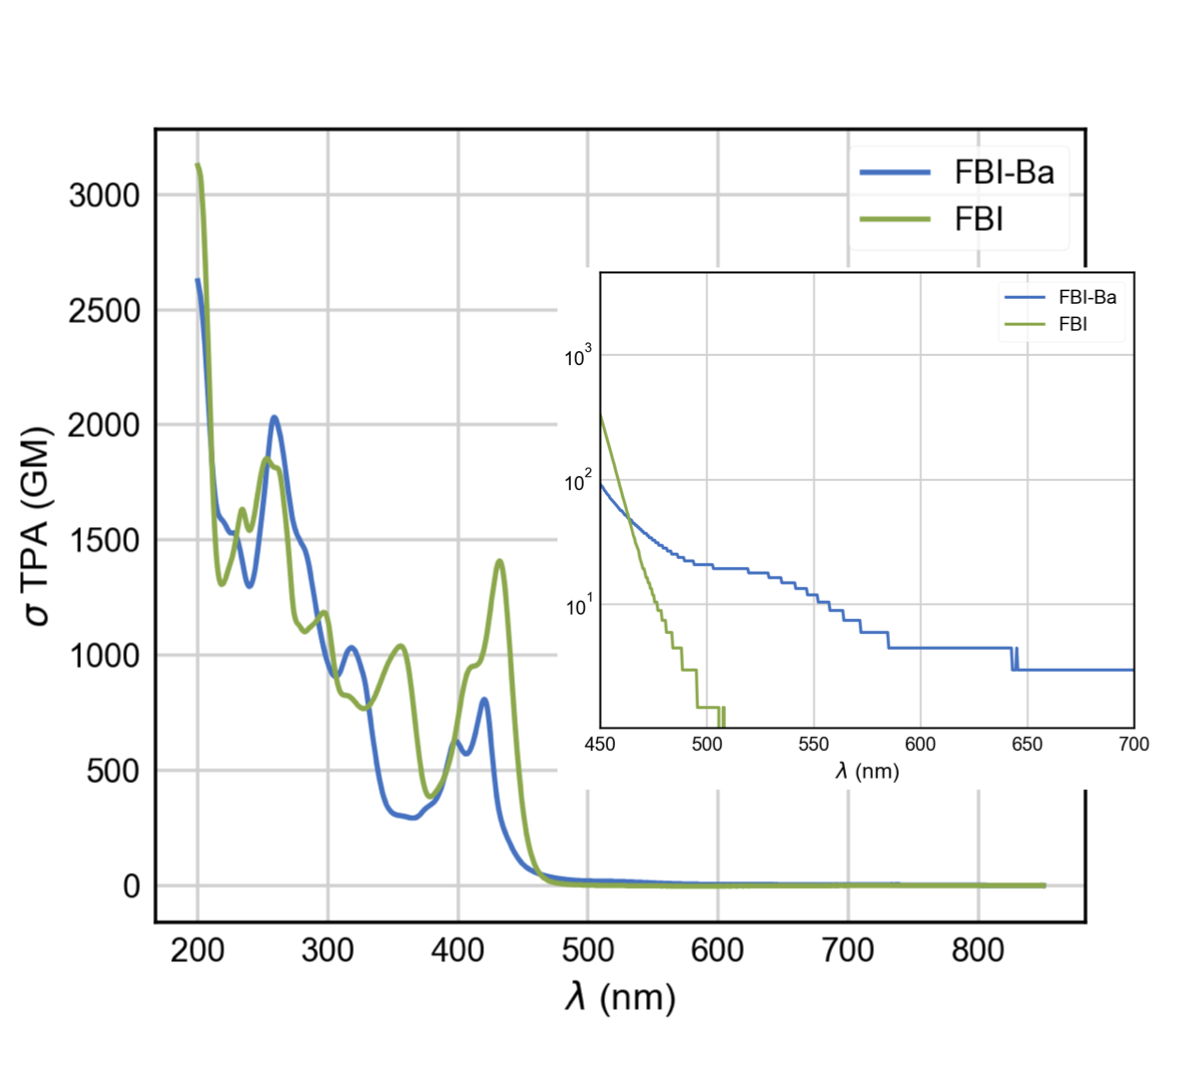
\includegraphics[width=0.95\textwidth]{figures/2PA_absospect.png}
	\caption{\label{absorSpectrum} Two-Photon Absorption cross section for FBI and FBI-Ba. Inset: zoom in the range of laser wavelength.}
\end{figure*}

The number of absorbed photons in a monolayer located on the beam focus is:

\begin{equation}
    N_{\mathrm{abs}} = \frac{1}{2}\rho_s \pi r_{\mathrm{fov}} \sigma_{\mathrm{TPA}} I^2,
\end{equation}

where:
\begin{itemize}
    \item $\rho_s \approx$ 1 nm$^{-2}$ is the surface density of molecules,
    \item $r_{\mathrm{fov}}$ = 660 nm is the radius of the Field of View in the diffractive limit.
    \item  $\sigma_{\mathrm{TPA}} $ is the TPA cross section at the wavelength of interest calculated above.
    \item $I$ is the flux of incident photons.
\end{itemize}

Notice the exponent 2 in the intensity of incident photons to account for the second-order effect and the 1/2 factor to account for the fact that two photons must be absorbed. Then, the number of re-emitted photons is just

$$N_{\mathrm{em}} = Q N_{\mathrm{abs}}, $$

where $Q$ is the fluorophore quantum yield, which has an estimated value of 0.25. Finally the number of detected photons must take into account the total efficiency of the setup:

$$N_{\mathrm{det}} = N_{\mathrm{em}} \varepsilon. $$

The setup efficiency must take into account the transmission rate of the objective, the viewports, the coupling to the collection optical fiber, and the dichroic mirror. Assuming the following values at 650 nm,
\begin{itemize}
    \item $\varepsilon_{APD} = 1$,
    \item $\varepsilon_{OB} = 0.87$,
    \item $\varepsilon_{filters} = 0.99$,
    \item $\varepsilon_{quartz} = 0.9$,
\end{itemize}

we can estimate the predicted number of photons that would be detected at the APD in the absence of quenching by the substrate. Figure \ref{detectedPhotons} represents this number as a function of the incident laser power.

\begin{figure*}[ht!]
	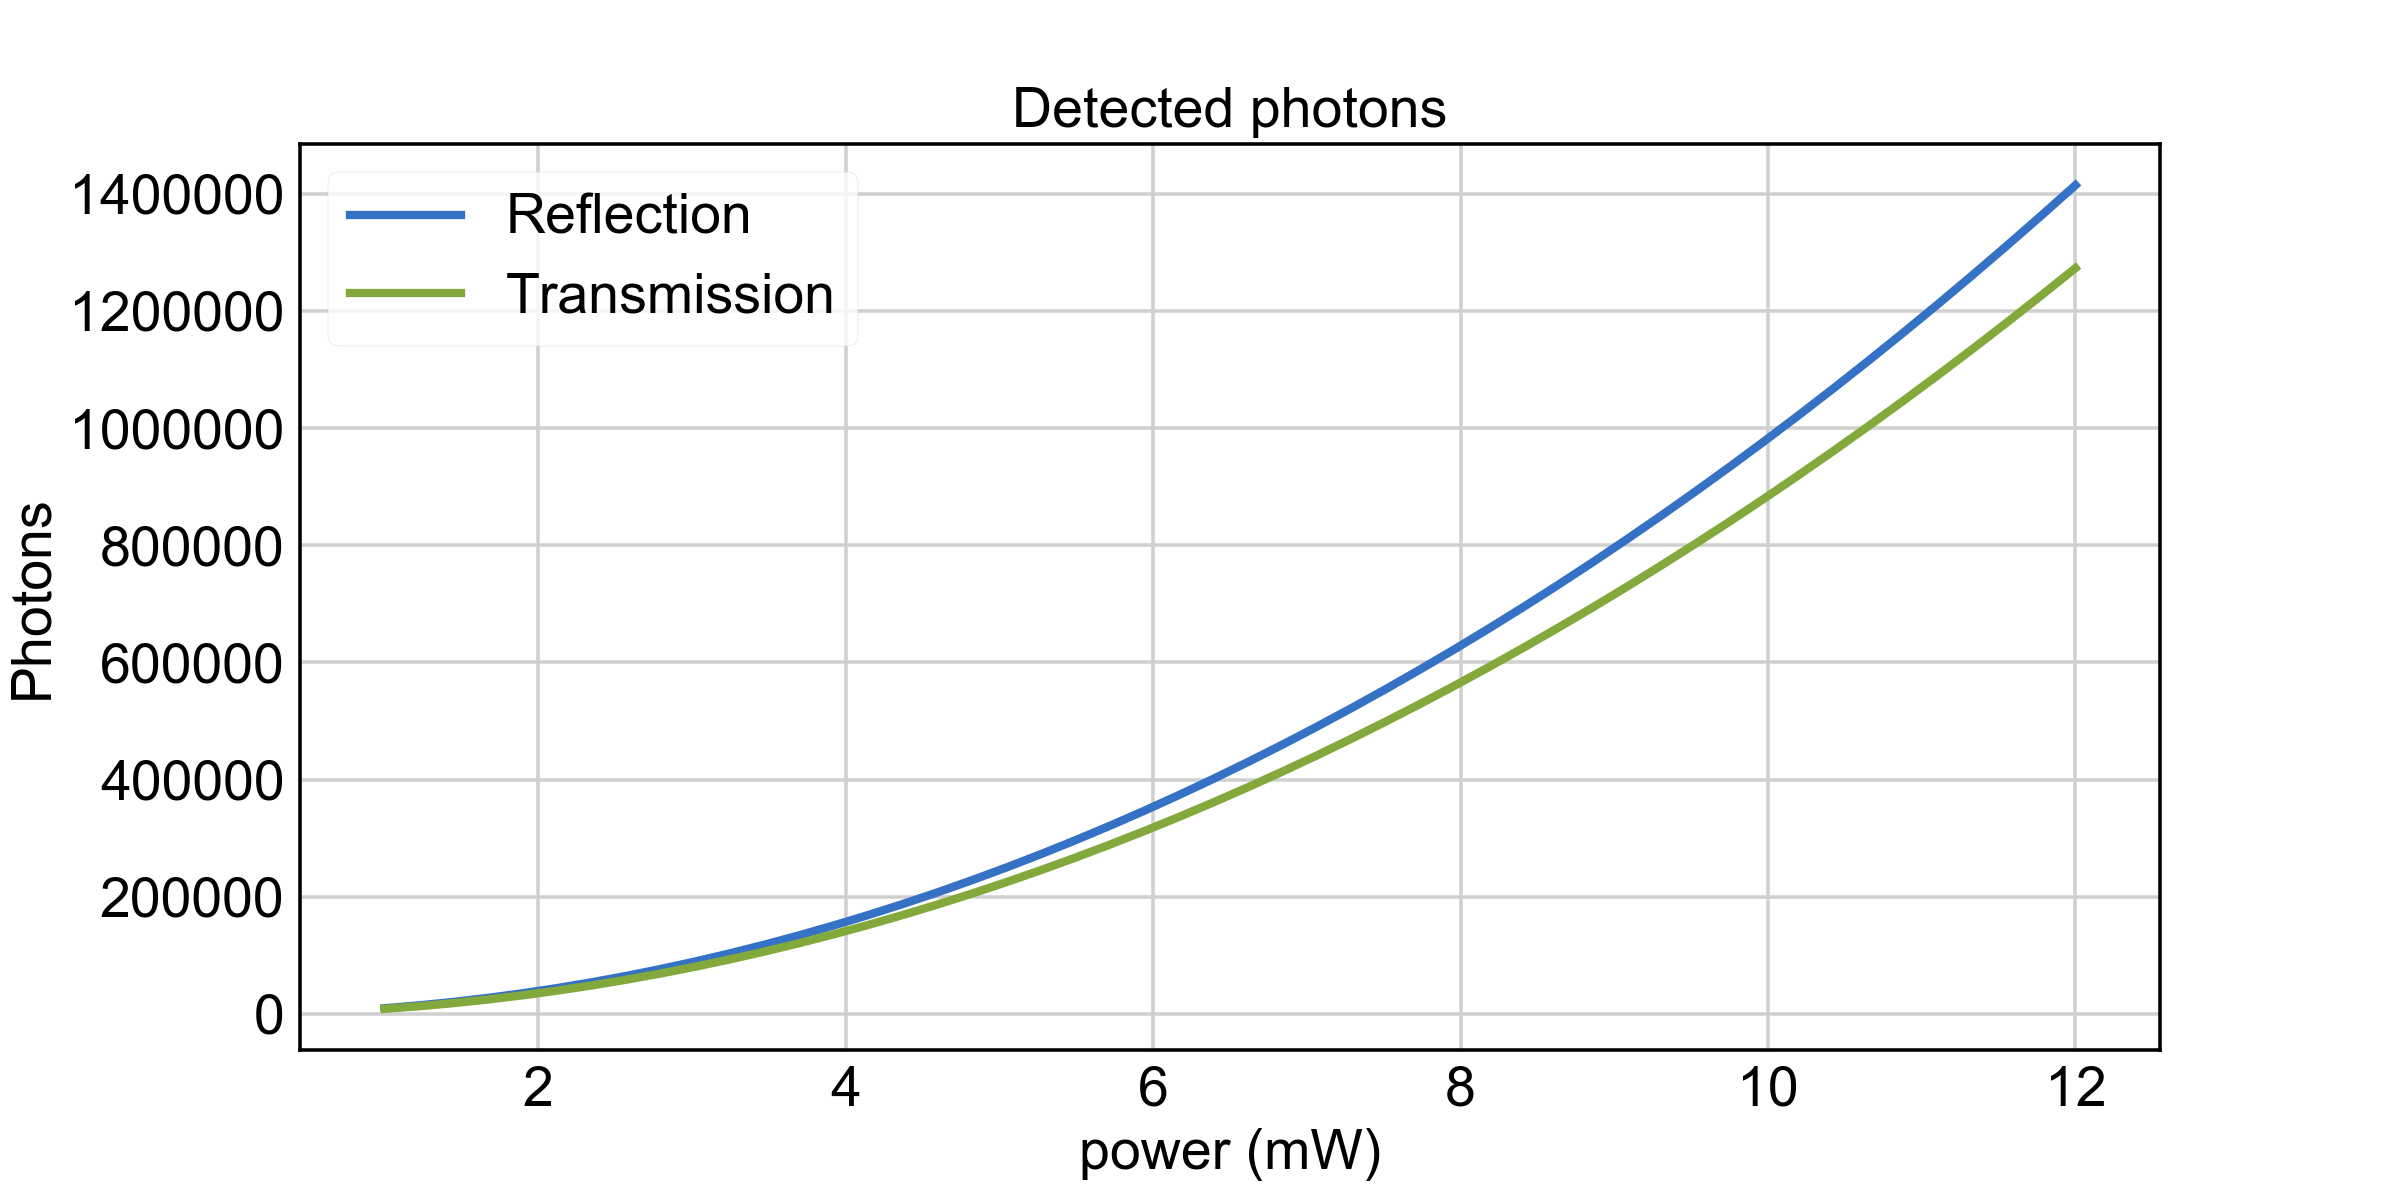
\includegraphics[width=0.95\textwidth]{figures/detectedPhot.png}
	\caption{\label{detectedPhotons} Expected number of photons detected by the APD.}
\end{figure*}

The curve for transmitted light is 0.9 times less intense as it takes into account the transmission through the quartz substrate.
\bibliographystyle{apsrev4-1}
\bibliography{sources}

\end{document}
